\section{From 2D Video to 3D Video}
\label{sec:intro_v2_background}

Over the past three decades, video has evolved from a specialized media format into a fundamental mode of communication over the Internet. 
%
On-demand services deliver large catalogs to geographically distributed audiences, live-streaming platforms carry events as they unfold, and video-conferencing systems support interactive conversations among participants separated by geographic distance.
%
This transition was enabled by the maturation of an entire ecosystem of components: inexpensive displays and cameras, efficient video codecs, broadband access networks, bitrate adaptation, and hardware-accelerated processing. 
%
Together, these components made it possible to capture, compress, transport, and render visual information at global scale.

The next step in this evolution is \textit{volumetric video}. 
%
A conventional video frame records the projection of a scene onto a two-dimensional image plane. 
%
The viewpoint is fixed when the frame is captured; a viewer may enlarge or crop the image, but cannot observe the scene from a new perspective. 
%
A volumetric video (also called 3D video) instead represents the geometry and appearance of a scene in three dimensions (3D). 
%
When viewed through an augmented-reality (AR) or virtual-reality (VR) display, this representation allows a viewer to walk and turn within the video and to observe the scene from any desired viewpoint (just like we perceive real world with our eyes and body), which gives full immersion and presence. 
%
Check~\cref{fig:vv_viewpoints} that shows 3 distinct viewpoints of the same frame from a volumetric video.
%
This ability to move along three translational and three rotational axes is commonly called \textit{six degrees of freedom} (6-DoF).

The distinction between 2D and 3D video is consequential. A two-dimensional video call can show a remote collaborator, whereas a volumetric call can place a three-dimensional representation of that collaborator and the surrounding workspace inside a shared virtual environment. 
%
A two-dimensional broadcast can choose a camera angle on behalf of every viewer, whereas a volumetric broadcast can allow each viewer to choose a position and perspective independently.
%
These capabilities can support richer forms of applications such as remote education~\cite{volumetric:education}, volumetric movies~\cite{volumetric:filmmaking}, tele-medicine and tele-surgery~\cite{volumetric:telemedicine}, cultural storytelling~\cite{volumetric-museology}, and sports broadcasting~\cite{volumetric-golf,volumetric-sports}.
%
A major application in this domain is volumetric telepresence, where multiple participants can interact with each other in a shared virtual space or real captured space in 6 degrees of freedom (6-DoF).
%
Participants can have the illusion that they are all in the same room instead of simply seeing 2D renderings of each other (\cref{fig:telepresence}).

\begin{figure}[t]
    \centering
    \begin{subfigure}[t]{0.32\textwidth}
        \centering
        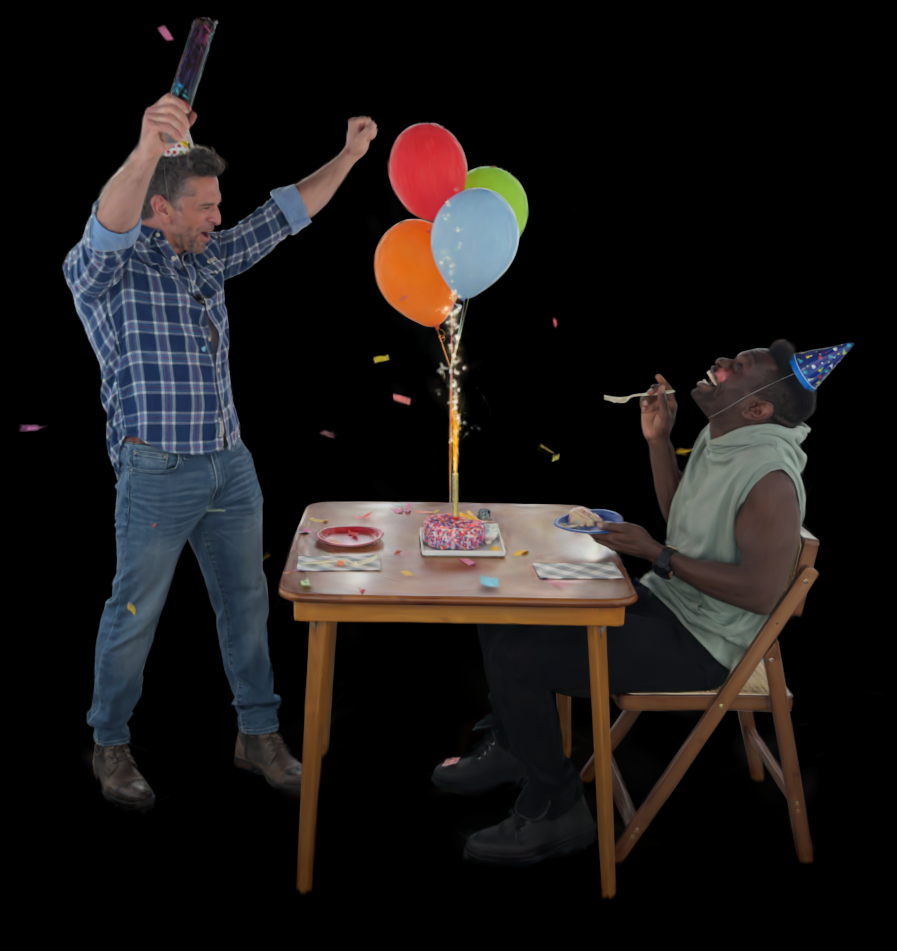
\includegraphics[width=\textwidth]{figures/view1.png}
    \end{subfigure}
    \hfill
    \begin{subfigure}[t]{0.32\textwidth}
        \centering
        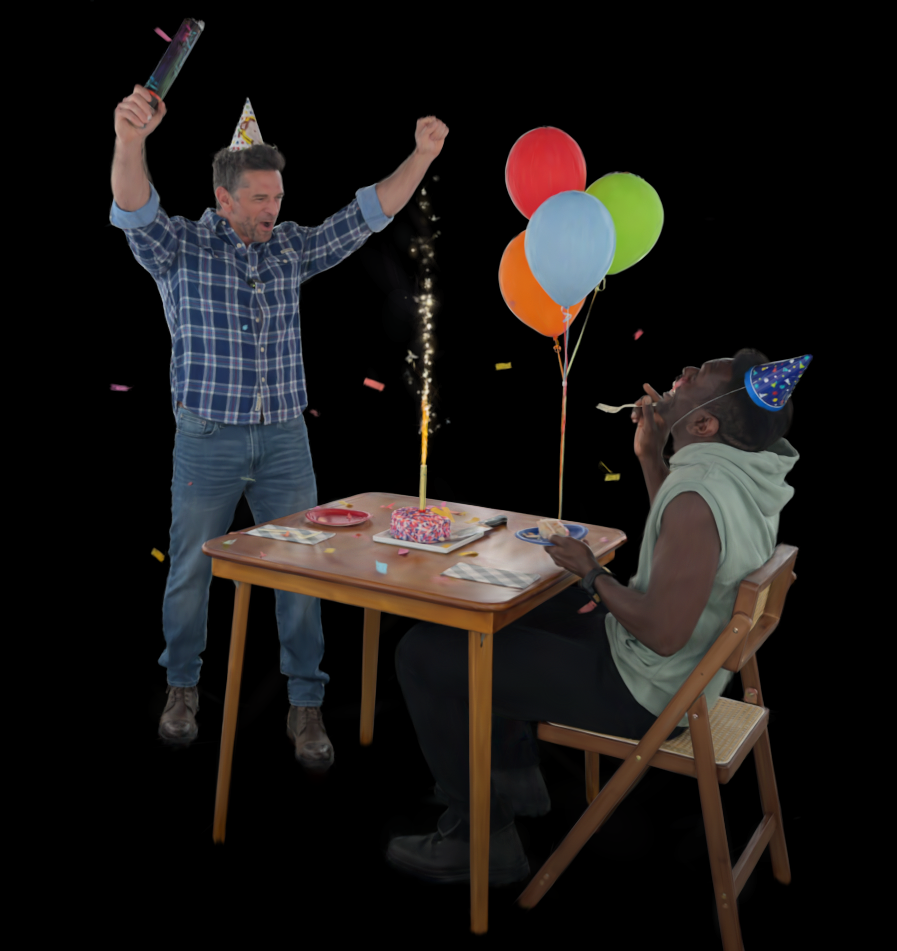
\includegraphics[width=\textwidth]{figures/view2.png}
    \end{subfigure}
    \hfill
    \begin{subfigure}[t]{0.32\textwidth}
        \centering
        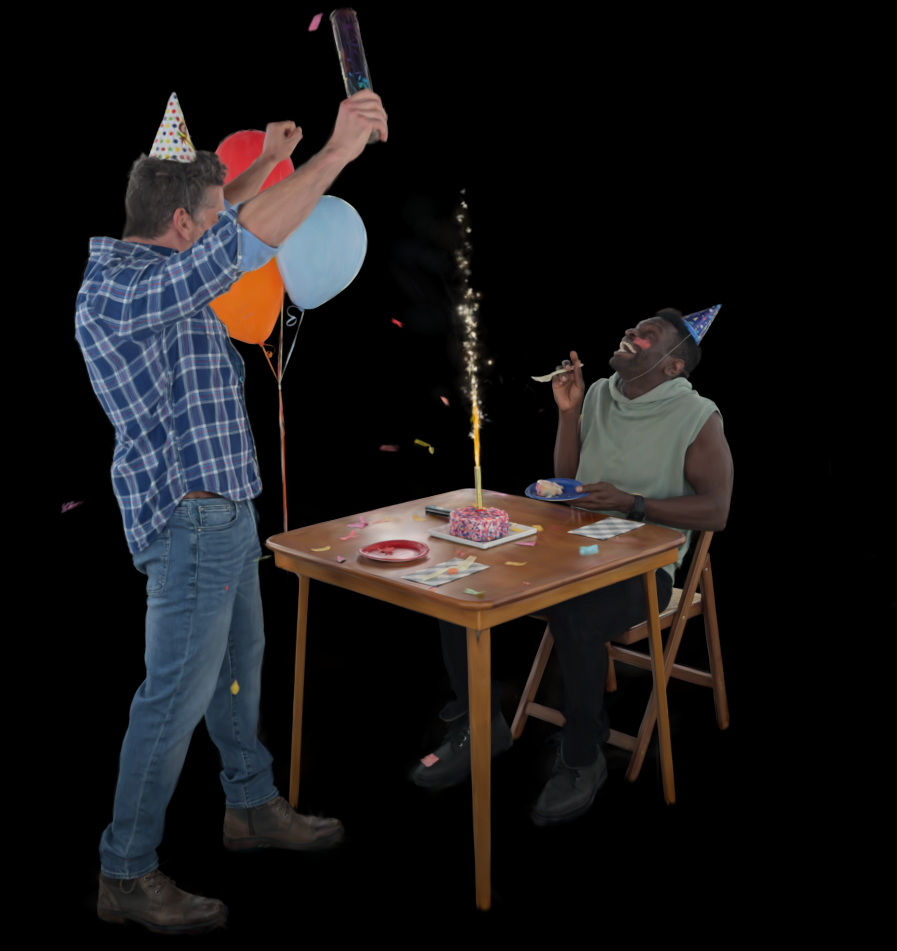
\includegraphics[width=\textwidth]{figures/view3.png}
    \end{subfigure}
       \caption{3 distinct viewpoints of a frame from a volumetric video~\cite{volumetric:gracia-example}.}
       \label{fig:vv_viewpoints}
\end{figure}

\begin{figure}[t]
    \centering
    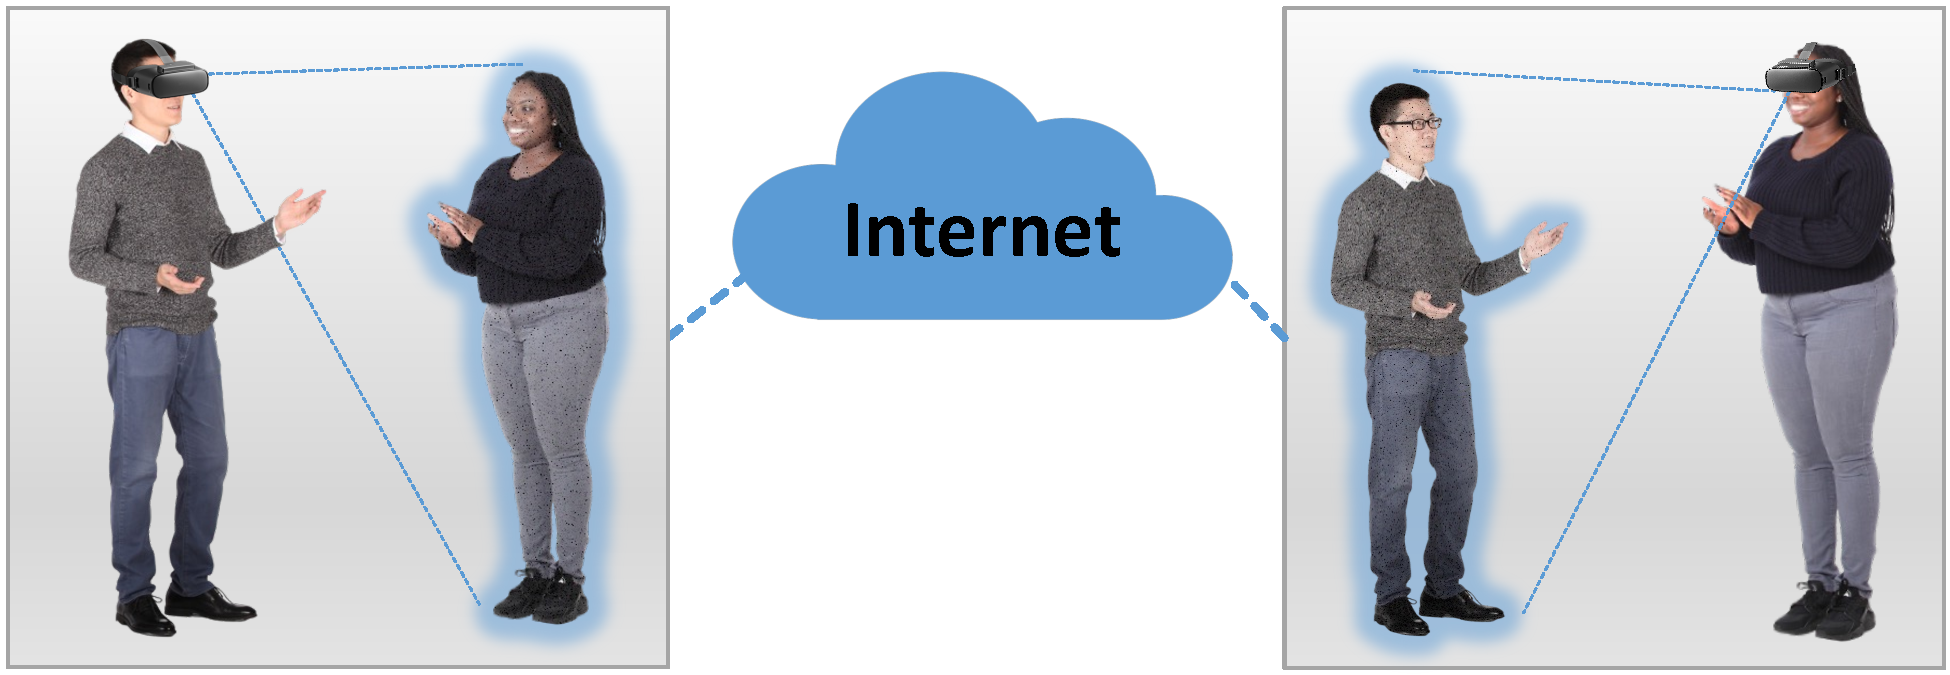
\includegraphics[width=\textwidth]{figures/AR-Depiction-0620.pdf}
    \caption{A telepresence session between 2 participants using volumetric video.}
    \label{fig:telepresence}
\end{figure}

\parab{Capturing and Representing Volumetric Video.}
%
Volumetric content can be captured in several ways.
%
An array of RGB-D cameras directly measures color and depth from multiple viewpoints. 
%
The depth measurements can be back-projected into three-dimensional space and fused into a \textit{point cloud}, in which each point records a position and visual attributes such as color.
%
Multi-camera images can also be processed into a mesh, whose vertices and faces describe surfaces, or used to learn a neural scene representation.
%
Neural Radiance Fields (NeRFs)~\cite{nerf} and 3D Gaussian Splatting (3DGS)~\cite{gsplat} are prominent examples of the latter approach.
%
In particular, 3DGS represents a scene using a set of oriented Gaussian primitives with geometry, appearance, and opacity attributes, and can render novel views at interactive rates.

These representations occupy different points in a broad design space.
%
Point clouds are straightforward to construct from depth cameras and are well suited to live capture, but they may contain holes or reveal sparsity when viewed from viewpoints close to objects.
%
Meshes provide explicit surfaces, but constructing and compressing dynamic meshes can be expensive.
%
Learned representations can produce photorealistic views, but training and transporting them introduce substantial computation and data volume.
%
The choice of representation is therefore not merely a rendering decision: it determines what information must traverse the network, which compression tools can be used, and whether an end-to-end system can operate in real-time.

\parab{Conferencing, Live Streaming, and On-demand Delivery.}
%
The delivery setting imposes an additional set of constraints.
%
An on-demand service can encode content beforehand, store multiple quality levels, and allow a client to fetch and buffer several seconds of data. 
%
A one-way live stream must process content as it is generated, but can often retain a modest playback buffer.
%
Conferencing is the most stringent case: it is bidirectional, and delays directly affect human interactivity.
%
Contemporary two-dimensional conferencing systems consequently target approximately 200--300~ms of end-to-end latency while processing video at frame rate~\cite{videoconf-benchmark,salsify,converge-sigcomm-2023,rfec-acm-mm2022}.

Volumetric delivery inherits all of these requirements while operating on substantially larger and less regular data. 
%
It must preserve three-dimensional geometry as well as appearance; it must account for a viewer whose position and orientation may change; and it must do so under network bandwidth that varies over time. 
%
Although point-cloud standards and codecs such as G-PCC~\cite{gpcc}, V-PCC~\cite{vpcc}, and Draco~\cite{draco} provide important compression capabilities, their encoding and decoding costs, compression behavior, and interfaces were not originally designed for the tight control loop of interactive, full-scene 3D data communication.

\parab{Technology Trends.}
Several trends make this an opportune time to revisit the volumetric delivery pipeline. 
%
Commodity RGB-D sensors can capture synchronized color and depth at high frame rate.
%
Broadband access rates are approaching the range needed for compressed full-scene content~\cite{cisco_whitepaper}, and modern video codecs expose direct bitrate control and hardware acceleration. 
%
At the same time, programmable GPUs have become ubiquitous on servers and increasingly capable on mobile and embedded devices. 
%
Finally, head-mounted and spatial displays are moving volumetric content from laboratory demonstrations toward practical applications.
%
The central question is therefore shifting from whether a three-dimensional scene can be captured and rendered to whether it can be \textit{communicated} with the efficiency, adaptivity, and responsiveness as expected of today's Internet video.

This dissertation addresses that question through two complementary systems.
%
\livo examines full-scene volumetric \textit{conferencing}, where the dominant requirements are direct adaptation to available bandwidth and low end-to-end latency at interactive frame rate.
%
\gsnfs examines frame-rate compression of dynamic Gaussian splats and point clouds, providing a native 3D video codec suitable for emerging live-streaming and on-demand delivery pipelines and perhaps also conferencing in future.
%
Together, they support the thesis of this dissertation: volumetric video can become a practical Internet medium when representation, compression, network adaptation, and computation are designed as parts of a single end-to-end system.

\section{A Vision for Immersive Conferencing and Live Streaming}
\label{sec:intro_v2_vision}
%
This dissertation envisions an Internet in which a dynamic three-dimensional scene can be communicated as readily as a two-dimensional video is communicated today.
%
At one end of the spectrum, two distant participants should be able to enter a shared session, move within their local spaces, and see each other's environments with 6-DoF and conversational latency.
%
At the other end, a lecture, performance, or sporting event should be captured once and delivered live to many viewers, each of whom can select a viewpoint.
%
In both cases, volumetric content should respond gracefully to changes in network capacity and should be decodable on the devices available to viewers.

Realizing this vision requires a pipeline with five tightly coupled stages.
%
First, a capture system observes a dynamic scene and constructs a sequence of 3D frames.
%
Second, an encoder exploits spatial and/or temporal redundancy and selects a quality that is compatible with the available rate.
%
Third, the network transports the resulting bitstream while bandwidth and delay vary.
%
Fourth, the receiver decodes the bitstream in real-time and reconstructs the dynamic 3D scene.
%
Finally, a renderer generates the view corresponding to the user's current viewpoint.
%
A decision made at any one stage affects the others.
%
For example, aggressive geometry compression reduces network load but can displace surfaces, distort color after reprojection, and ultimately reduce immersion.
%
Likewise, a representation that renders efficiently may still be impractical if its attributes cannot be encoded and decoded at frame rate.

\section{Challenges}
\label{sec:intro_v2_challenges}

The vision above exposes several challenges that distinguish volumetric communication from conventional video.
%
These challenges are coupled: reducing data volume can increase computation or reduce visual quality, while improving fidelity can make real-time delivery infeasible. 

\begin{table}[t]
    \begin{center}
   {%\footnotesize
     % \scalebox{0.7}
     {
     \begin{tabular}{|l|l|l|l|l|l|l|}
       \hline
       \textbf{Compression} & \textbf{\begin{tabular}[c]{@{}l@{}}Type of \\ Compression\end{tabular}} & \textbf{\begin{tabular}[c]{@{}l@{}}Bandwidth-\\ adaptive?\end{tabular}} & \textbf{Latency (ms)} \\ \hline
       Draco~\cite{draco} & 3D & \crossmark & 100 - 300 \\ \hline
       G-PCC~\cite{gpcc} & 2D & \checkmark & 1000 - 5000 \\ \hline
       V-PCC~\cite{vpcc} & 2D & \checkmark & > 60000 \\ \hline
       \rowcolor{Gainsboro!60} \livo & 2D & \checkmark & < 30 \\ \hline
       \rowcolor{Gainsboro!60} \gsnfs & 3D & \checkmark & < 30 \\ \hline
       \end{tabular}
     }
   }
     \caption{Comparison of different compression techniques for volumetric video.}
     \label{tab:compression_challenges}
   \end{center}
\end{table}

\parab{Data Volume.}
A volumetric frame contains geometry in addition to appearance and can describe an entire physical environment rather than a single camera projection. 
%
In the datasets used by \livo, an uncompressed full-scene point-cloud frame can exceed 10~MB. 
%
At 30~frames per second, a 10~MB frame corresponds to roughly 2.4~Gbps before compression. 
%
The scale is even larger for learned representations: a 3DGS frame with one million Gaussians can require approximately 236~MB because each Gaussian carries more than just color.
%
Compression is therefore unavoidable.

\parab{Bandwidth Adaptation.}
Compression alone is insufficient as available bandwidth changes rapidly. 
%
An on-demand player can often absorb short-term variation with a buffer; an interactive volumetric session cannot accumulate a large buffer without harming conversation. 
%
The encoder must select a rate that fits current capacity, and it must revise that choice as conditions change. 
%
This control problem is particularly difficult when a 3D codec exposes only indirect quality parameters rather than a target bitrate. 
%
\livo addresses direct adaptation by using rate-adaptive 2D codecs, whereas \gsnfs supplies fast encode/decode primitives and rate--distortion flexibility on which a native adaptive controller can be built, while competing schemes still aren't directly bandwidth-adaptive; refer to~\cref{tab:compression_challenges}.

\parab{Interactive Latency and Frame-rate Processing.}
A 30 fps pipeline receives a new frame about every 33~ms. 
%
Although different stages can be pipelined, none can fall persistently behind this arrival rate. 
%
Conferencing further requires capture, encoding, network transport, decoding, and rendering to fit within an end-to-end target of a few hundred milliseconds. 
%
A codec that achieves excellent compression but takes seconds to encode a frame is unsuitable for this setting. 
%
Current state-of-the-art 3D codecs fall in this category; refer to~\cref{tab:compression_challenges}.
%
Likewise, a receiver that cannot decode at frame rate will either stall or accumulate delay.

\parab{Visual Fidelity under Compression.}
Errors in volumetric data are perceived differently from errors in an image. 
%
A color error changes appearance at a fixed location; a depth or geometry error moves the location itself and can also move the color attached to it. 
%
Point-cloud sparsity may produce holes or expose floating points as a viewer changes perspective. 
%
More photorealistic representations such as 3DGS improve novel-view rendering, but attach many correlated attributes to every primitive and consequently increase the compression burden. 
%
A volumetric system must therefore allocate bits across geometry and appearance according to their perceptual impact, not simply minimize the error of a flattened two-dimensional representation.

\section{Contributions}
\label{sec:intro_v2_contributions}

\begin{figure}[t]
    \centering
    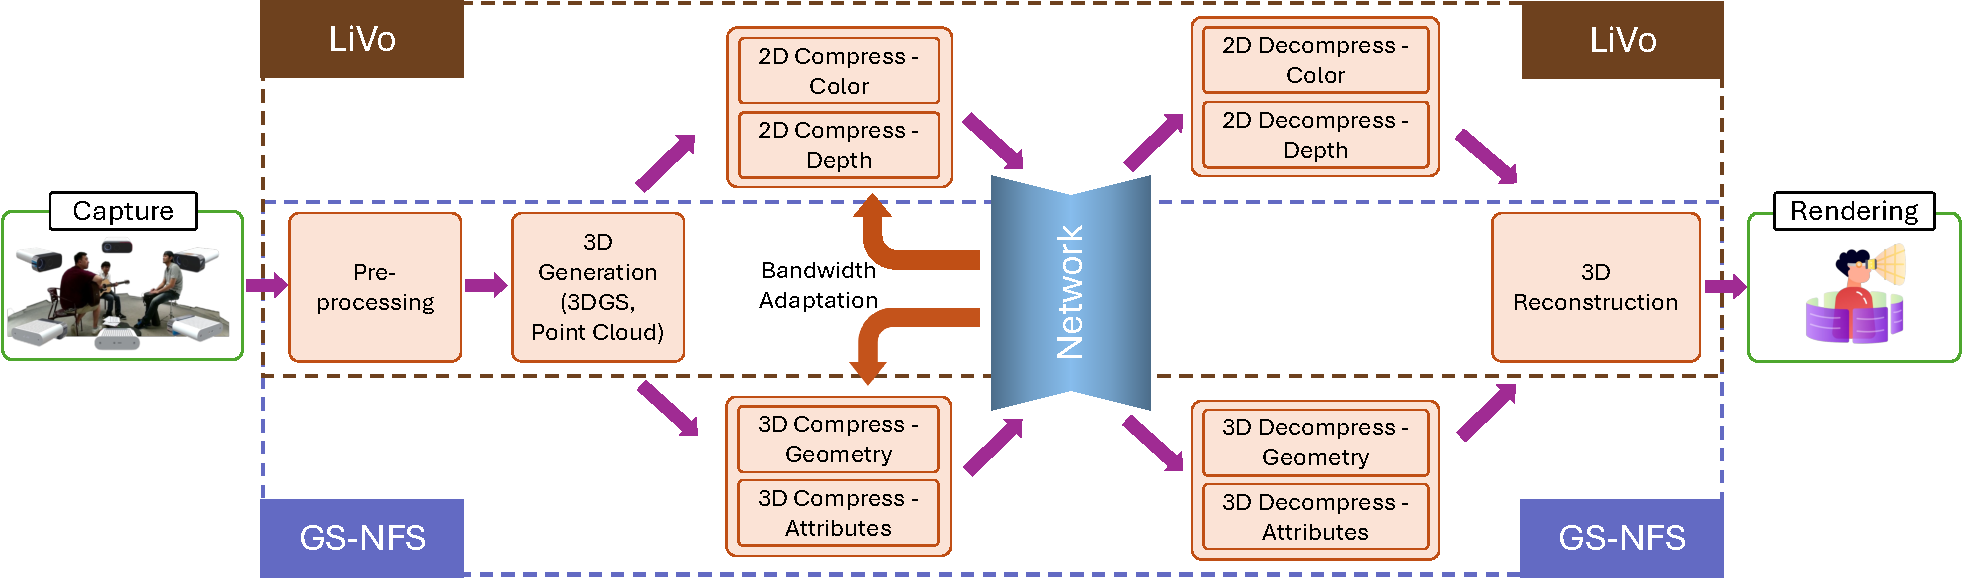
\includegraphics[width=\textwidth]{figures/thesis_pipeline.pdf}
    \caption{The dissertation's vision for volumetric communication. \livo and
    \gsnfs address complementary paths through a common end-to-end delivery pipeline.}
    \label{fig:thesis_pipeline}
\end{figure}

This dissertation takes two steps toward the vision of practical volumetric communication.
%
\cref{fig:thesis_pipeline} illustrates how these two systems approach the pipeline. 
%
\livo asks how far a volumetric conferencing system can progress by reusing the mature infrastructure of 2D video.
%
Its sender retains the RGB-D organization of the captured data, composes the color and depth observations into two video streams, and uses rate-adaptive 2D codecs and WebRTC to transport them.
%
The receiver reconstructs a point cloud and renders the view selected by the user.
%
This approach makes bandwidth adaptation and hardware-accelerated compression immediately available, but requires new mechanisms to preserve depth, divide bandwidth between geometry and appearance, and avoid transmitting portions of the scene that a receiver cannot see.

\gsnfs explores a complementary path motivated by the rapid improvement of native 3D representations. 
%
It compresses dynamic 3DGS frames after training, using an architecture derived from point-cloud coding but redesigned so that the entire pipeline can execute on a GPU. 
%
The same pipeline can encode point clouds because both representations consist of spatial primitives with associated attributes. 
%
This generality creates a bridge between the two systems. 
%
A future \livo-like system could construct point clouds at the sender and use \gsnfs, or a rate-adaptive codec derived from it, in place of a 2D color/depth path or substantially slower 3D codecs. 
%
Such an integration is not evaluated in this dissertation, but it demonstrates why fast native 3D compression is relevant not only to Gaussian-splat delivery, but also to the broader evolution of volumetric streaming and conferencing.

\subsection{Bandwidth-adaptive Volumetric Conferencing with \livo}
\label{sec:intro_v2_livo}

\livo, presented in \cref{ch:livo}, enables two-way conferencing between full physical spaces. 
%
Each site uses an array of RGB-D cameras to observe the local scene. 
%
Rather than first constructing a point cloud and then invoking a slow conventional 3D codec, \livo preserves the camera observations as color and depth images, composes them into two large video streams (one for each color and depth), and transports those streams using WebRTC. 
%
The receiver decodes the images, reconstructs a point cloud, and renders it from the user's current viewpoint. 
%
This architecture deliberately inherits the bandwidth efficiency, direct rate control, and hardware acceleration of mature 2D video codecs.

Reusing 2D codecs solves only part of the problem. 
%
Full-scene depth spans a larger physical range than portrait-style telepresence, and depth errors displace geometry in the reconstructed scene. 
%
Moreover, color and depth are carried in separate streams and compete for the same network capacity. 
%
Finally, sending an entire scene wastes bits on geometry that lies outside the receiver's field of view. 
%
\livo addresses these issues through three main contributions:

\squishlist
    \item \textbf{Full-scene color and depth encoding.} \livo multiplexes observations from multiple RGB-D cameras into a color stream and a depth stream. It develops a depth representation that preserves a wide physical depth range while remaining compatible with efficient video encoding. This stream composition limits receiver-side synchronization and permits the codec to exploit redundancy across camera observations.

    \item \textbf{Adaptive bandwidth splitting.} A fixed division of network capacity between color and depth is suboptimal because scene complexity and available bandwidth change over time. \livo monitors the distortion of the encoded streams and dynamically assigns bandwidth between them, giving depth sufficient protection when geometry distortion would dominate perceived quality.

    \item \textbf{Pose-aware view prediction and culling.} \livo predicts the receiver's near-future viewing frustum from recent 6-DoF poses and removes observations that will not be visible. It performs this operation on the RGB-D images before point-cloud construction, reducing both the data presented to the encoder and the computation required for culling.
\squishend

\livo demonstrates that this combination can meet conferencing constraints for full-scene content. 
%
In evaluations using real user-viewing traces and time-varying network traces, it sustains approximately 30~fps with around 250~ms of end-to-end latency. 
%
A user study and objective point-cloud quality measurements show that \livo consistently improves perceived and measured quality relative to baseline schemes. 
%
These results establish that mature 2D video infrastructure with careful design choices can serve as a practical substrate for immersive two-way communication.

\subsection{Frame-rate 3D Compression with \gsnfs}
\label{sec:intro_v2_gsnfs}

\gsnfs, presented in \cref{ch:gsnfs}, addresses the codec bottleneck for a different class of volumetric representations. 
%
A dynamic \gs video, or \dgs, contains a sequence of Gaussian-splat frames. 
%
Each frame is a set of gaussian primitives whose attributes describe position, scale, rotation, opacity, and view-dependent color. 
%
The representation can render high-quality novel views quickly, but an uncompressed frame may contain hundreds of megabytes of attributes.
%
Existing post-training approaches map these attributes into 2D video or extend CPU-oriented point-cloud codecs~\cite{v3volumetric,mesongs,LTS,gpcc}. They provide useful compression, but their encoding or decoding costs can prevent frame-rate operation.

\gsnfs starts from the observation that a Gaussian-splat frame resembles a point cloud
with a richer attribute vector. 
%
It therefore adopts the broad structure of G-PCC: positions are represented using an octree, attributes are transformed using RAHT, the resulting coefficients are quantized, and the bitstream is entropy-coded. 
%
Its central departure is to keep this entire pipeline on the GPU. 
%
Doing so requires eliminating explicit tree traversal and exposing parallelism despite the irregular distribution of the primitives.
%
\gsnfs makes three principal contributions:

\squishlist
    \item \textbf{Parallel octree encoding and decoding.} \gsnfs uses Morton codes to impose a spatial order on primitives and to derive parent--child relationships without pointer-based traversal. It processes the implicit octree level by level, enabling nodes at the same level to be encoded or decoded concurrently on the GPU.

    \item \textbf{Parallel attribute transformation.} \gsnfs reformulates RAHT around Morton-ordered active elements and parallel operations at each hierarchy level. It couples this transform with GPU-resident quantization and entropy coding, avoiding repeated transfers between CPU and GPU memory.

    \item \textbf{Compression efficiency.} Gaussian-splat color is represented by spherical-harmonic coefficients whose components exhibit substantial correlation. \gsnfs transforms the coefficients from RGB to YUV and applies a Karhunen--Lo\`eve transform (KLT) to the AC coefficients before RAHT, reducing redundancy with little additional execution time.
\squishend

On desktop GPUs, \gsnfs encodes evaluated dynamic Gaussian-splat frames in approximately 18--23~ms and decodes them in approximately 14--21~ms, meeting a 30~fps frame budget and improving substantially on the latency of evaluated post-training baselines. 
%
Its compression performance is better than several point-cloud-derived alternatives and is competitive with a 2D-video-based approach on large full-scene sequences. 
%
On a Jetson Orin, \gsnfs decodes some sequences at up to approximately 25~fps.
%
To demonstrate real-time performance, \gsnfs is combined with a feed-forward Gaussian generator and it can encode and decode the frames at line rate.

Although \gsnfs is motivated by \gs or \dgs delivery, its octree and attribute coding stages operate on spatial points with associated attributes. 
%
It can consequently serve as a native point-cloud codec with only the attribute configuration changed. 
%
This creates a path for a future conferencing system to replace slow, indirectly controlled 3D codecs with a GPU-resident alternative, while retaining the low-latency capture and transport principles developed in \livo.

\parab{Combined Contribution.}
Taken together, the two chapters show that volumetric delivery benefits from innovation at both the systems and codec layers. 
%
\livo begins with a deployment constraint---today's 3D codecs do not simultaneously provide the speed and direct bitrate control required for conferencing---and constructs a practical path through 2D video infrastructure. 
%
\gsnfs revisits that constraint and demonstrates that a native 3D pipeline can be restructured to approach frame-rate performance on desktop and mobile-class GPUs. 
%
\livo therefore establishes how to close the end-to-end conferencing loop today, while \gsnfs expands the set of representations and codec architectures that future live volumetric systems can employ.

\section{Dissertation Organization}
\label{sec:intro_v2_organization}

The remainder of this dissertation is organized as follows:

\squishlist
    \item \cref{ch:livo} presents \livo, a bandwidth-adaptive system for full-scene volumetric video conferencing. It describes the use of tiled color and depth streams, adaptive bandwidth splitting, receiver-view prediction and culling, and an evaluation of visual quality and end-to-end performance.

    \item \cref{ch:gsnfs} presents \gsnfs, a GPU-resident post-training codec for dynamic Gaussian splats and point clouds. It develops parallel octree and RAHT algorithms, improves attribute compression through color decorrelation, and evaluates frame-rate performance, rate--distortion behavior, mobile decoding, and live 3D use cases.
    
    \item \cref{ch:related} presents relevant literature in volumetric video generation, compression, delivery, and quality assessment.
    
    \item \cref{ch:conclusion} concludes the dissertation and discusses future work.
\squishend

Together, these chapters progress from an immediately deployable conferencing architecture built on 2D video infrastructure to a native 3D codec designed for the representations and delivery systems of the next generation.
